\begin{figure*}[t]
\centering
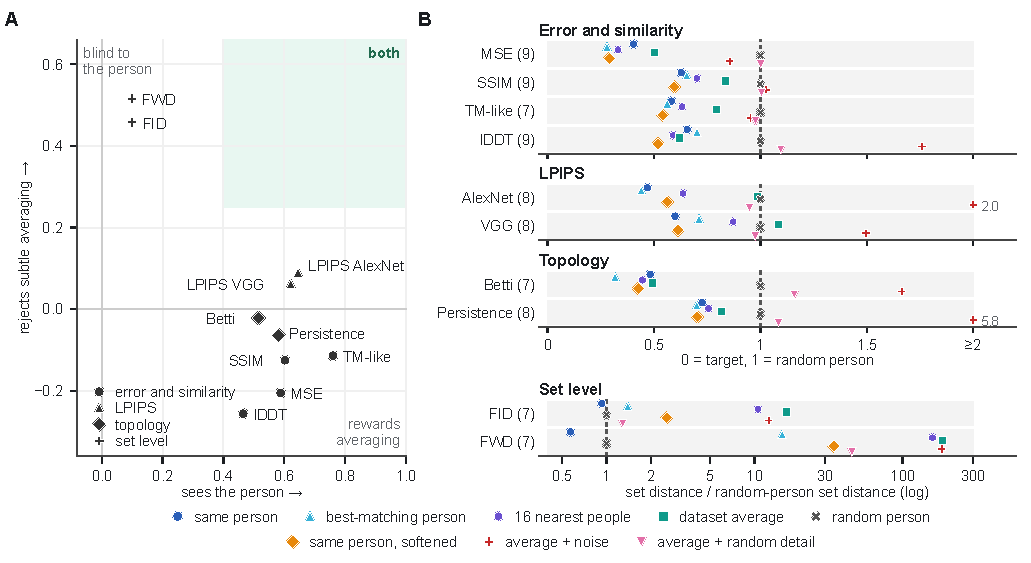
\includegraphics[width=\textwidth]{fig/metric_summary_v7.pdf}
\caption{\textbf{Pixel metrics see the person, set-level metrics reject averaging, and no metric does both.}
\textbf{A,} One point per metric.
x (RQ1): how far beyond the same person the metric places a random person; y (RQ2): how far beyond the unchanged same person it places the softened same person; both are rank differences along the ladder divided by the number of rungs, averaged over image sets.
The shaded corner would hold a metric that answers both, and none falls there.
\textbf{B,} Each fill on the random-person scale (0 = target, 1 = average of 16 random people), averaged over the image sets where it exists (in brackets); fixed lanes in legend order, rungs in cool and controls in warm colors.
\acs{FID} and \acs{FWD} are set distances divided by the random-person set's distance, on a log axis.
The sibling is omitted (2 of 9 image sets record families); \acs{TM}-like needs second images, so PAPILA and IXI have no value.
QTIM is left out of the \acs{LPIPS} and persistence averages and brain out of the Betti and set-level averages; brain, retina and iris are provisional.
Under \acs{MSE} the same person sits at 0.40, the softened same person at 0.29 and the dataset average at 0.50, while \acs{FID} and \acs{FWD} put the dataset average 16 and 186 times as far as a random person yet leave the same person near a random person.}
\label{fig:summary}
\end{figure*}
% Source: results/cross_modality/fig_metric_summary_R.json; drawn by src/cross_modality/summary_figure_v7.py (v4 figure kept as fig/metric_summary.pdf).
